\chapter{Introducción específica} % Main chapter title
\label{Chapter2}

%----------------------------------------------------------------------------------------
% Resumen de capitulo
%----------------------------------------------------------------------------------------

En el presente capítulo se describe el estado actual de algunas soluciones implementadas, y se elige una plataforma existente, que cumple con los requerimientos del trabajo como base. También, se presenta el estudio del código fuente de \textit{Arm Mbed OS Simulator}. 

%----------------------------------------------------------------------------------------
\section{Estado del arte}
\label{sec:Estado del arte}
%----------------------------------------------------------------------------------------

Hoy en día no existe una herramienta de emulación para la placa EDU-CIAA-NXP. Sin embargo, existe la plataforma de código abierto ViHard \citep{ViHard} que emula dispositivos de hardware en la PC, pero con la placa ECU-CIAA-NXP real conectada a la PC a través del puerto USB. En la figura \ref{fig:ViHard} se muestra el esquema de la plataforma ViHard.

\begin{figure}[ht]
	\centering
	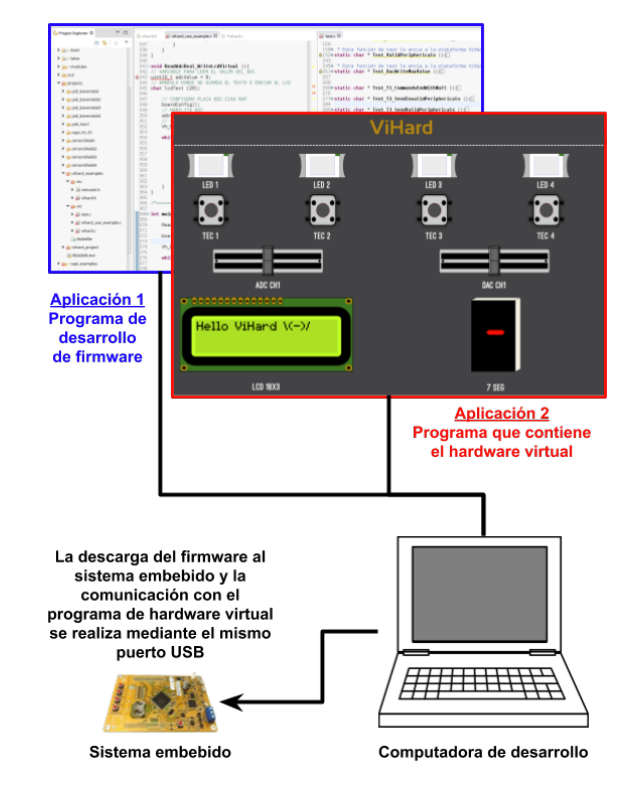
\includegraphics[scale=.40]{./Figures/ViHard.png}
	\caption{Esquema de la plataforma ViHard.\protect\footnotemark}
	\label{fig:ViHard}
\end{figure}

La plataforma se compone de un programa de PC con los perifericos virtuales de hardware y una biblioteca de firmware para la EDU-CIAA-NXP, que controla y gestiona el funcionamiento del hardware virtual. Ambos programas se comunican con el sistema embebido mediante UART, a través de un puerto USB.

El programa de hardware virtual es una aplicacion de escritorio multiplataforma desarrollada utilizando el framework Electron \citep{Electron}. Por otro lado, la biblioteca embebida fue desarrollada en lenguaje C. 

Por lo tanto, el usuario necesita ejecutar en su PC el programa de periféricos virtuales y contar con la biblioteca en el sistema embebido que controla el hardware virtual. A partir de ahí, procedería al desarrollo de su propio programa, que deberá compilar y descargar a la EDU-CIAA-NXP, y posteriormente realizar las pruebas correspondientes.

Por otro lado, se encontraron muchas plataformas educativas que simulan microcontroladores, sobre todo para la placa Arduino \citep{Arduino}. Para el análisis, se seleccionaron algunos de los simuladores más populares que implementan funcionalidades relevantes para el presente trabajo, los cuales se describen en las siguientes secciones. 

%------------------------------------
\subsection{UnoArduSim}

UnoArduSim \citep{UnoArduSim} fue desarrollado en la Universidad de Queen \citep{Queensu} por el profesor Stan Simmons. En la figura \ref{fig:UnoArduSim} puede observarse la interfaz del programa.

\begin{figure}[ht]
	\centering
	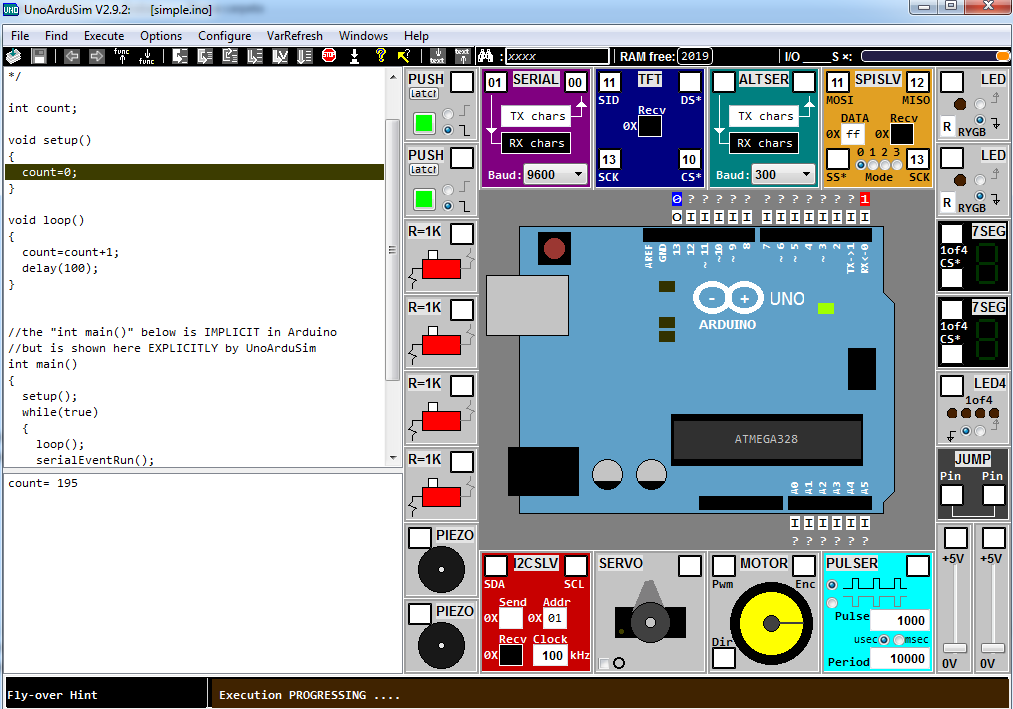
\includegraphics[scale=.33]{./Figures/UnoArduSim.png}
	\caption{Plataforma UnoArduSim.}
	\label{fig:UnoArduSim}
\end{figure}

La herramienta simula en la pantalla de la PC la placa Arduino Uno \citep{ArduinoUno} y muchos de los dispositivos de entrada y salida más usados, asimismo, permite la depuración interactiva de funciones o programas completos. Está diseñada específicamente para ejecutarse en el sistema operativo Windows. Además, el diseño de la interfaz gráfica no promueve la claridad visual, puesto que hay demasiados objetos en la pantalla y los que existen deberían estar mejor distribuidos. 

%------------------------------------
\subsection{Virtronics}

Virtronics \citep{Virtronics} es uno de los simuladores más completos que hay hoy en día para Arduino \citep{Arduino}, ya que permite simular varios modelos y, además, tiene dos versiones disponibles: una versión paga y otra gratuita, pero con funciones limitadas. En la figura \ref{fig:Virtronics} se muestra la plataforma.

\begin{figure}[ht]
	\centering
	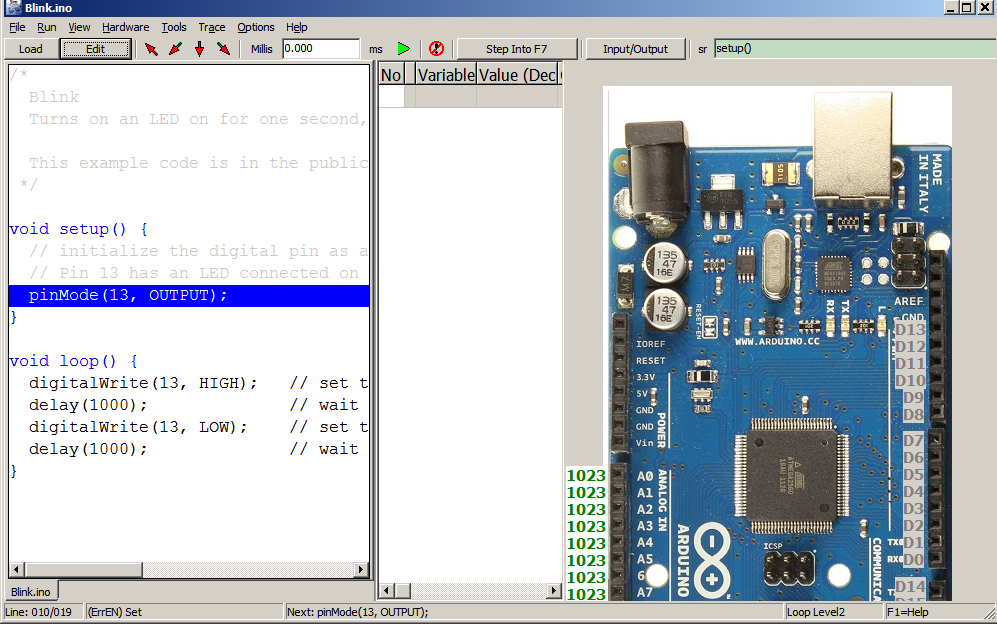
\includegraphics[scale=.35]{./Figures/Virtronics.png}
	\caption{Plataforma Virtronics.}
	\label{fig:Virtronics}
\end{figure}

%------------------------------------
\subsection{Tinkercad}

Tinkercad \citep{Tinkercad} es una plataforma online que permite el acceso desde cualquier navegador web, cuya interfaz de usuario se muestra en la figura \ref{fig:Tinkercad}.

\begin{figure}[ht]
	\centering
	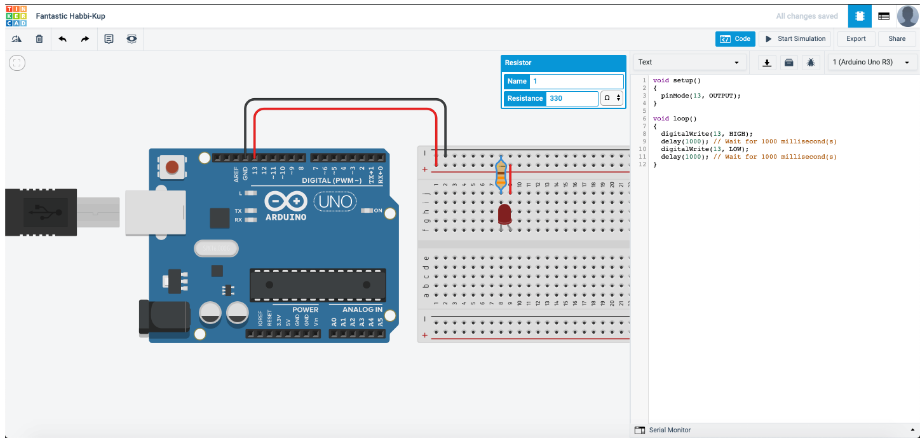
\includegraphics[scale=.40]{./Figures/Tinkercad.png}
	\caption{Plataforma Tinkercad.}
	\label{fig:Tinkercad}
\end{figure}

Fue desarrollado por ingenieros y diseñadores de software de Autodesk \citep{Autodesk} y permite diseños 3D. Adicionalmente, es necesario crear una cuenta  antes de empezar a usar la plataforma, por consiguiente, todos los diseños se guardan en la cuenta creada. 

%------------------------------------
\subsection{\textit{Arm Mbed OS Simulator}}

\textit{Arm Mbed OS Simulator} \citep{ArmMbedSim} fue desarrollado por ingenieros de Arm, encargados de mantener las bibliotecas Mbed OS, \citep{ArmMbed} y es parte de Mbed Labs. La plataforma era accesible \textit{on line} al momento del comienzo de este proyecto, pero actualmente debe ser descargado desde su repositorio [ref] y luego, puede ejecutarse utilizando cualquier navegador web en la red local, o bien, realizar el despliegue en un servidor para que esté disponible \textit{on line}. En la figura \ref{fig:ArmMbed} puede observarse la plataforma online de Mbed Simulator.

\begin{figure}[ht]
	\centering
	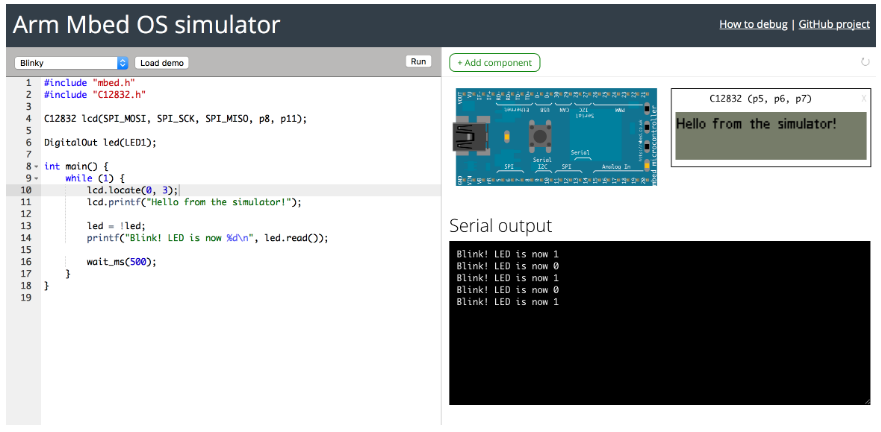
\includegraphics[scale=.44]{./Figures/ArmMbed.png}
	\caption{Plataforma Arm Mbed OS Simulator.}
	\label{fig:ArmMbed}
\end{figure}

El funcionamiento de este emulador es muy simple. Se puede crear un programa desde cero, o bien, se puede elegir un ejemplo de la lista desplegable y cargar el proyecto desde el botón \textquotedbl Load demo\textquotedbl, luego añadir los componentes necesarios para el programa, como por ejemplo, el display que se observa en la figura \ref{fig:ArmMbed}, donde se pide al usuario indicar a qué pines estará conectado. Es importante mencionar que el programa ya incluye la placa con el microcontrolador precargada. Una vez completo el programa y el ensamblado del hardware, se puede compilar y ejecutar en el emulador usando el botón \textquotedbl Run\textquotedbl.

%----------------------------------------------------------------------------------------
\section{Análisis de los emuladores revisados}
\label{sec:Análisis de los emuladores revisados}
%----------------------------------------------------------------------------------------

En la tabla \ref{tab:simuladores} se comparan las características más importantes de estos emuladores. 

\hfill \break
\hfill \break
\hfill \break
\hfill \break
\hfill \break
\hfill \break
\hfill \break
\hfill \break
\hfill \break

\begin{table}[ht]
\centering
\caption[Comparación de características de los emuladores revisados]{Comparación de características de los emuladores revisados}
\begin{tabular}{p{0.24\linewidth} p{0.17\linewidth}  p{0.19\linewidth}  p{0.14\linewidth}  p{0.10\linewidth}}
\toprule
\textbf{Característica} 
& \textbf{UnoArduSim}
& \textbf{Virtronics}
& \textbf{Tinkercad}
& \textbf{Mbed OS}
\\
\midrule
Placa/Plataforma emulada & Arduino Uno & Varios modelos Arduino & Arduino Uno & Arm Mbed OS\\
Gratuito &    Sí & No & Sí & Sí\\
Aplicación & Escritorio & Escritorio & Web & Web\\
Plataforma & Windows & Windows/Linux & Todas & Todas\\
Código abierto & No & No & No & Sí\\
Dispositivos E/S & Sí & Sí & Sí & Sí  \\
Panel de desarrollo & Sí & Sí & Sí & Sí \\
Lenguaje & C & C & C & C/C++\\
Debugging & Sí & Sí & Sí & No\\
Ejemplos & Sí & Sí & Sí & Sí\\
\bottomrule
\hline
\end{tabular}
\label{tab:simuladores}
\end{table}

Cabe destacar, que de las plataformas revisadas \textit{Arm Mbed OS Simulator} es la única de código abierto. Sin embargo, este análisis sirve tembién para revisar, comprender y comparar las ventajas y desventajas de las otras plataformas, y tomar características útiles para el desarrollo del emulador. 

Del análisis anterior, se desprende que \textit{Arm Mbed OS Simulator} presenta las siguientes ventajas significativas:

\begin{itemize}
	\item Código abierto: al tener acceso al código fuente permitió estudiar cómo funciona internamente el proyecto simulador, además, de la libertad de uso y distribución.
	\item Arquitectua de aplicación web. 
    \item Su capacidad para simular dispositivos y componentes.
	\item Comunidad y Soporte: el proyecto tiene una comunidad activa de desarrolladores, que brinda acceso a una amplia base de conocimientos, documentación y soporte. 
	\item Reconocimiento de Marca ARM mbed OS: al basarse en su proyecto simulador, se puede obtener cierto reconocimiento y confianza entre los usuarios.
	\item Reutilización: ofrece un conjunto sólido de funcionalidades y características ya probadas que agilizó el desarrollo y redujo la probabilidad de introducir errores.
	\item Actualizaciones y Mejoras Continuas: el proyecto Mbed Simulator recibe actualizaciones continuas con las últimas tecnologías que permite mantener el emulador para la placa EDU-CIAA-NXP actualizado.	
\end{itemize}

Sim embargo, actualmente, \textit{Arm Mbed OS Simulator} presenta las siguientes limitaciones:

\begin{enumerate}
	\item Dentro de un bucle infinito \texttt{while(1)}, es necesario agregar un retraso \newline(\texttt{delay)}, de lo contrario, el navegador no puede actualizar la interfaz de la plataforma web ni responder a eventos del usuario. Esto significa que el navegador no tiene la oportunidad de realizar otras tareas o responder a eventos mientras el bucle está en ejecución. Como resultado, el navegador se bloquea o congela y puede dejar de responder.
	
	\item En cada iteracion, la ejecución del programa puede variar en términos de tiempo, lo que puede afectar a la precisión en la sincronización de eventos dentro de la aplicación.

	\item En \textit{Arm Mbed OS Simulator}, no hay restricciones significativas en cuanto a la cantidad de memoria que se puede asignar al stack o al heap  de un programa, lo cual difiere del hardware físico, donde sí existen limitaciones de memoria.
	
	\item Dentro del entorno web, las interrupciones no se manejan de la misma manera que en un sistema embebido real, debido a que no implementa el manejo de prioridades, por lo cual no afectan la ejecución del programa principal.
	
	\item Sin RTOS. No tiene la capacidad de ejecutar múltiples hilos de manera concurrente como lo haría un RTOS. Todo el código se ejecuta en un solo hilo. Se puede utilizar la biblioteca mbed-events para manejar ciertos aspectos de concurrencia, usando eventos y temporizadores.
	
	\item Emulación a nivel API de Mbed OS. No permite programar a bajo nivel, utilizando registros de core para la arquitectura ARM o periféricos.
	
	\item Sin capacidad de debug paso a paso. Se realiza el programa, se compila y ejecuta en el hardware virtual pero no permite la depuración de código.
\end{enumerate}

Dadas todas estas consideraciones y una vez confirmada su compatibilidad para los propósitos del presente trabajo, se decide basar el emulador de la EDU-CIAA-NXP en portar el proyecto \textit{Arm Mbed OS Simulator}, para la EDU-CIAA-NXP y sus bibliotecas.

%----------------------------------------------------------------------------------------
\section{Análisis del código fuente de \textit{Arm Mbed OS Simulator}}
%----------------------------------------------------------------------------------------

Se procedió a analizar en detalle el código fuente de \textit{Arm Mbed OS Simulator} para adquirir una compresión de su arquitectura, del funcionamiento del \textit{Sistema Operativo Mbed}, de los periféricos simulados y sus las interacciones, así como de las configuraciones necesarias para la plataforma web.

%------------------------------
\subsection{Análisis de las tecnologías utilizadas}

\textit{Arm Mbed OS Simulator} es una aplicación web. Este tipo de aplicaciones son provistas por un servidor web y pueden ser accedidas por los usuarios que se conecten a través de internet desde cualquier lugar mediante un navegador web \citep{NavegadorWeb}. Además, presentan la arquitectura cliente/servidor (que se muestra en la figura \ref{fig:ClienteServidor}) en donde un cliente o navegador web realiza peticiones al servidor y en consecuencia el servidor envía la respuesta de regreso.

\begin{figure}[ht]
	\centering
	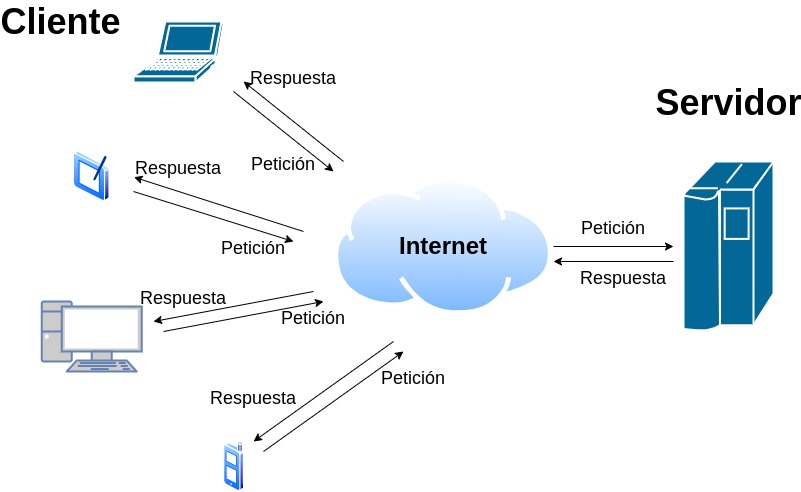
\includegraphics[scale=.48]{./Figures/EsquemaCliente_Servidor.jpg}
	\caption{Esquema modelo cliente/servidor.}
	\label{fig:ClienteServidor}
\end{figure}

\hfill \break
\hfill \break
\hfill \break

Las razones por las que se optó por la tecnologia web se debe a las potenciales ventajas que presentan, de las cuales las más importantes son:

\begin{itemize}
	\item No es necesario instalar nada en la computadora del usuario.
	\item No consumen los recursos del ordenador.
	\item No se encuentra limitado a un lugar físico específico para acceder y utilizar las capacidades de emulación.
	\item No obliga al usuario usar un determinado sistema operativo, ya que se puede ejecutar en todos los dispositivos con acceso a un navegador web y una conexión a internet.
\end{itemize}

En el desarrollo web, el \textit{frontend} es la parte del software que interactúa con el usuario y el \textit{backend} es la parte lógica que se encarga de tomar los datos, procesarlos y devolverlos al \textit{frontend}. En la figura \ref{fig:frontBackMbed} se muestra un esquema con las tecnologías web usadas en el presente trabajo.

\hfill \break
\hfill \break
\hfill \break
\hfill \break
\hfill \break
\hfill \break
\hfill \break
\hfill \break
\hfill \break
\hfill \break
\hfill \break
\hfill \break

\begin{figure}[ht]
	\centering
	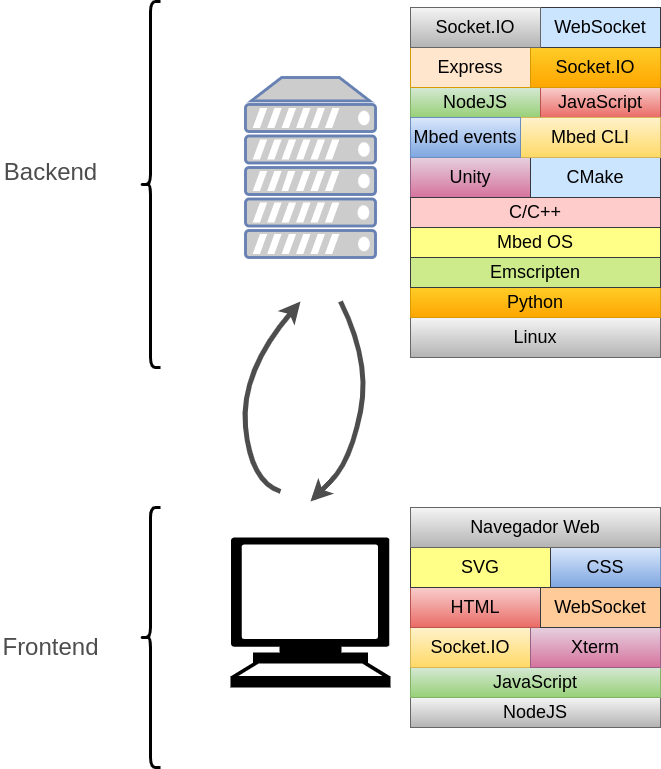
\includegraphics[scale=.47]{./Figures/FrontendBackendMbed.png}
	\caption{Esquema de las tecnologías utlilizadas en \textit{Arm Mbed OS Simulator}.}
	\label{fig:frontBackMbed}
\end{figure}

En las siguientes secciones se describen las tecnologías que forman parte del \textit{frontend} y \textit{backend} del emulador.

%-------------------------
\subsection{Frontend}
\label{subsec:Frontend}

Se describen brevemente las principales tecnologías utilizadas:

\begin{itemize}
	\item JavaScript \citep{JavaScript}: es un lenguaje de programación que se ejecuta del lado del cliente en el navegador, o bien del lado del servidor mediante motores como NodeJS \citep{NodeJS}. En el caso del lado del cliente, permite crear páginas web dinámicas y también responder a eventos causados por el propio usuario tales como modificaciones del DOM, de la sigla en inglés  \textit{Document Object Model} \citep{DOM}. Por consiguiente, el desarrollo con JavaScript en el frontend permitió cargar y ejecutar los archivos resultantes generados por el compilador en el navegador. Asimismo, es el responsable de configurar el entorno necesario para ejecutar el emulador web y proporcionar la interfaz de usuario para la interacción. Además, en el backend fue útil para gestionar la comunicación y la interacción entre los diferentes componentes a través de solicitudes HTTP, permitiendo la transferencia de datos y el flujo de información dentro de la plataforma web.

	\item NodeJS \citep{NodeJS}: es un entorno de ejecución de JavaScript cuyo propósito es el desarrollo de aplicaciones web y servicios del lado del servidor. También, proporciona una arquitectura orientada a eventos y no bloqueante. 
De manera que, en el contexto del frontend, se utilizó como parte del flujo de trabajo de desarrollo, incluyendo la gestión de dependencias, automatización de tareas de compilación, pruebas y despliegue. Mientras tanto, en el backend, se utilizó para desarrollar las rutas, controladores y manejar la lógica de la aplicación en respuesta a las solicitudes entrantes y el envío de respuestas.

	\item HTML \citep{HTML}: de la sigla en inglés \textit{Lenguaje de Marcas de Hipertexto, del inglés HyperText Markup Language}, es el lenguaje de marcas que sirve para etiquetar contenido y visualizarlos en el navegador web.
	Este lenguaje es sencillo de aprender y es fácil de interpre­tar tanto por humanos como por máquinas.  En el desarrollo, se utilizó para crear los elementos visuales de la interfaz de usuario, como los botones, lista desplegable, pantallas de visualización, y otros componentes necesarios para interactuar con el emulador web.

	\item CSS \citep{CSS}: de la sigla en inglés \textit{Cascading Style Sheets},
	es un lenguaje de diseño gráfico que permite definir estilos, colores, formato, tamaño, tipo de letra del texto, posición de cada elemento dentro de la página, etc. Es la mejor forma de separar los contenidos y es necesario para crear páginas web complejas. El desarrollo con CSS ayudó a controlar la presentación visual y el estilo de la plataforma.

    \item SVG \citep{SVG}: de la sigla en inglés \textit{Scalable Vector Graphics}, es un formato de gráficos vectoriales bidimensionales con una base matemática que pueden modificarse según se necesite. Las imágenes creadas con este formato se pueden escalar y hacer zoom de forma arbitraria sin pérdida de resolución debido a que no están formadas por píxeles. Además, esta basado en el lenguaje de marcado extensible XML \citep{XML} y es un formato muy útil para ser utilizado en entornos web. 
Para el desarrollo del diseño de la interfaz fue ideal el uso de este tipo de formato para evitar que las imagenes se deformen y también, ofrecer una experiencia visual interactiva.

    \item Xterm \citep{Xterm}: es un componente escrito en TypeScript \citep{TypeScript} que permite que una aplicación pueda usar terminales emuladas con todas sus funciones en el navegador web. 
En el desarrollo del emulador web, se utilizó esta tecnología en la interfaz de usuario para visualizar la salida de la terminal.

    \item WebSocket \citep{WebSocket}: esta tecnología permite la comunicación bidireccional entre el cliente y el servidor, trabaja sobre el protocolo TCP/IP y también, es una especificación de protocolo de HTML5, de la sigla en inglés \textit{HyperText Markup Language, versión 5} \citep{HTML5}. 
Se utilizó WebSocket para establecer la comunicación entre el frontend y el backend, y de esta manera, permitir la transferencia de datos de manera dinámica con el fin de mostrarlos en la terminal serial del emulador. 
       
    \item Socket.IO \citep{Socket}: es una biblioteca de Javascript que usa websocket para la comunicación bidireccional y para la baja latencia. También, está basada en el manejo de eventos entre un cliente y un servidor. El desarrollo con esta tecnología facilitó la transmisión de eventos en tiempo real para la salida de los datos de la terminal serial.

\end{itemize}

%-------------------------
\subsection{Backend}

Se describen brevemente las principales tecnologías que se usaron en el backend.

\begin{itemize}
	\item Emscripten \citep{Emscripten}: es un compilador que traduce la mayor parte del lenguaje LLVM, de la sigla en inglés \textit{Low Level Virtual Machine} \citep{LLVM}, a JavaScript. De esta forma, permite ejecutar el código de varios lenguajes de programación en los navegadores actuales.
Emscripten compila C y C++ en WebAssembly \citep{WebAssembly} mediante LLVM y Binaryen \citep{Binaryen}. La salida de Emscripten puede ejecutarse en la web y en NodeJS.
El uso de esta herramienta tuvo por objetivo el compilar el código escrito en C, a WebAssembly (Wasm) y JavaScript.	Esto permitió ejecutar aplicaciones nativas en la web sin necesidad de plugins o complementos adicionales.

	\item Python \citep{Python}:  es un poderoso y popular lenguaje de programación multiplataforma de código abierto. Se caracteriza por su sencillez y su gran potencia para el tratamiento de datos en el lado del servidor. En el emulador web, Python se utilizó para escribir scripts que realizan tareas específicas, como la configuración e inicialización de la plataforma web del emulador.
    
    \item Express \citep{Express}: es un marco de aplicaciones web en el backend para NodeJS. También, está diseñado para crear aplicaciones web y APIs, de la sigla en inglés \textit{application programming interface} \citep{API}. Se utilizó Express para configurar middlewares que permiten servir archivos estáticos desde carpetas específicas, como \textquotedbl outUser \textquotedbl, que contiene los archivos generados por Emscripten.
    
    \item Lenguaje C \citep{LenguajeC}: es de propósito general y es muy popular debido al eficiente código que produce al crear software de sistemas y de aplicaciones. 
    Asimismo, es un lenguaje de tipos de datos estáticos, fuertemente tipado y tiene estructuras típicas de los lenguajes de alto nivel pero, a su vez, tiene construcciones que permiten un control de los lenguajes de bajo nivel. El desarrollo con C fue fundamental, ya que permitió la integración de la biblioteca sAPI del Proyecto  CIAA en el desarrollo del emulador web.
    
    \item Mbed CLI \citep{MbedCLI}: es una herramienta de línea de comandos que facilita el desarrollo y la gestión de proyectos basados en la plataforma Mbed \citep{ArmMbed}. Incluso, permite realizar tareas como la configuración del entorno de desarrollo, compilación de código, gestión de dependencias y la depuración, permitiendo identificar y resolver problemas en el código. Se reutilizó esta herramienta, ya incluída en el emulador sobre el cual se basó este trabajo, para proporcionar una interfaz de línea de comandos que simplificó las tareas de configuración y despliegue del emulador web.
 
    
     \item Mbed events \citep{ArmMbed}: es una biblioteca de código que se utiliza en el desarrollo de software embebido para facilitar la gestión de eventos y temporizadores. Para el desarrollo de la plataforma del emulador web se reutilizó esta biblioteca para la creación y gestión de tareas en el RTOS.
     
\end{itemize}

%------------------------------
\subsection{Análisis estructural de archivos y carpetas}

\begin{figure}[ht]
	\centering
	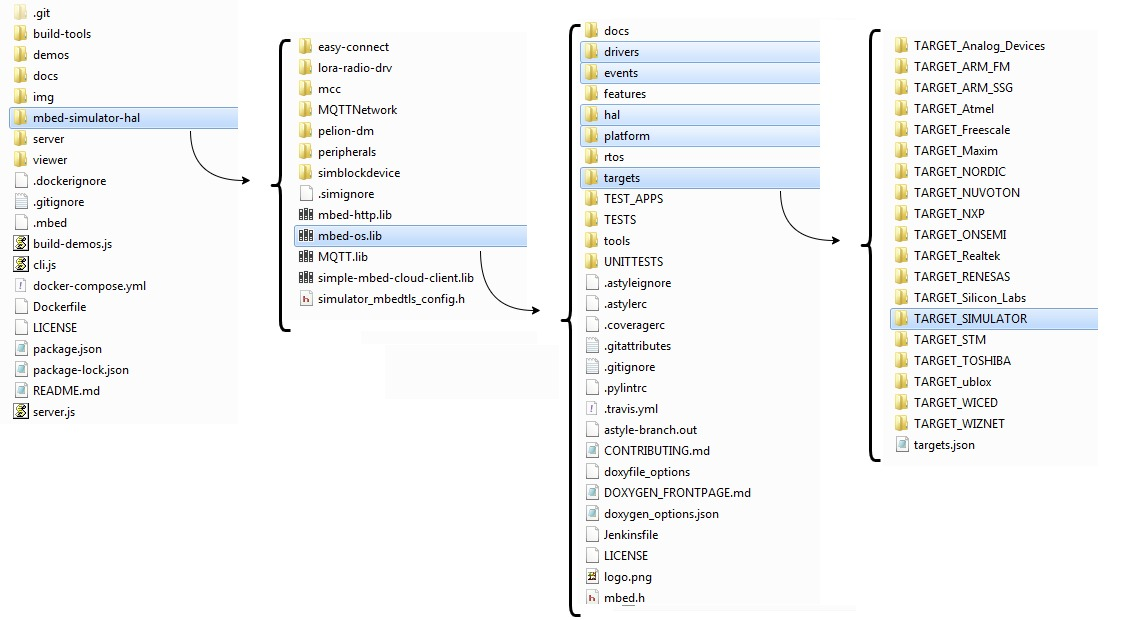
\includegraphics[scale=.37]{./Figures/estructuraMbed.jpg}
	\caption{Estructura de carpetas y archivos de \textit{Arm Mbed OS Simulator}.}
	\label{fig:estructuraMbed}
\end{figure}

En la figura \ref{fig:estructuraMbed} se exhibe la estructura de arbol de las carpetas y archivos de \textit{Arm Mbed OS Simulator} clonado desde GitHub.

\hfill \break
 
La carpeta \textquotedbl build-tools\textquotedbl{}  contiene tres archivos javascript: 

\begin{enumerate}
	\item build-application.js, que contiene funciones para construir aplicaciones en el contexto de \textit{Arm Mbed OS Simulator}. Asimismo, contiene métodos para encontrar los periféricos y manejar la construcción de componentes.
	
	\item build-libmbed.js, es un módulo de Node.js que realiza la compilación \textit{(build)} y gestión de dependencias. También, proporciona métodos que verifican las dependencias necesarias antes de la construcción.

	\item helpers.js,  es un módulo de Node.js que proporciona funciones relacionadas con operaciones de sistema de archivos, compilación, y manipulación de directorios y archivos.
\end{enumerate}
 
Dentro de la carpeta \textquotedbl demos\textquotedbl{}  se encuentran todos los programas ejemplo que muestran cómo utilizar ciertas funcionalidades de \textit{Arm Mbed OS Simulator} y son útiles como referencia para comenzar con el desarrollo en el entorno web. 
 
La carpeta \textquotedbl server\textquotedbl{}  contiene tres archivos javascript: 

\begin{enumerate}
	\item compile.js, este archivo realiza la generación de los archivos de salida compilados a partir del codigo fuente.
	
	\item get\_ips.js, proporciona una función para la configuración de las aplicaciones de red.

	\item launch-server.js, define y configura un servidor web que permite ejecutar solicitudes de ejecución de aplicaciones, gestionar las conexiones de red y la comunicación LoRaWAN.
	
\end{enumerate}
 
La carpeta \textquotedbl viewer\textquotedbl{}  contiene los archivos necesarios para crear interacción con el navegador. Entre estos archivos se encuentran: HTML, CSS, JavaScript, imágenes y bibliotecas de terceros o frameworks.
 
La carpeta \textquotedbl mbed-simulator-hal\textquotedbl{}  contiene las siguientes sub-carpetas y son usadas en el contexto de \textit{Arm Mbed OS Simulator}: 

\begin{itemize}
	\item easy-connect, dentro de esta carpeta se encuentran archivos que facilitan la conexión a una red utilizando Ethernet para manipular conexiones de red, sockets y eventos.
	
	\item lora-radio-drv, proporciona un marco para interactuar y controlar el módulo de radio LoRa, lo que permite enviar y recibir datos, administrar el estado y el funcionamiento.

	\item mcc, establece una cola de eventos que se utilizará para manejar eventos en \textit{Arm Mbed OS Simulator}. 
	
	\item MQTTNetwork, establece la interfaz para la comunicación de red con el protocolo MQTT. 
	
	\item pelion-dm, implementación de temporizadores y manejo de eventos para la plataforma mbed.
	
	\item peripherals, proporciona implementación de los periféricos externos para ejecutarse en el entorno web.
	
	\item simblockdevice, establece una interfaz para interactuar con  dispositivos de bloques que emula un dispositivo de almacenamiento físico en el navegador web.
	
	\item mbed-os.lib, es un archivo de biblioteca en formato binario que contiene la versión del código fuente del sistema operativo de Mbed OS  que usa \textit{Arm Mbed OS Simulator}.
	
\end{itemize}

La biblioteca \textquotedbl mbed-os.lib\textquotedbl{} se compone de las siguiente carpetas: 

\begin{itemize}

	\item drivers, dentro de esa carpeta se encuentran los diversos controladores que interactúan con los periféricos de hardware, y además, proporcionan una interfaz para acceder a ellos. 
	
	\item events, presenta archivos relacionados con la infraestructura de manejo de eventos para las tareas y operaciones de manera asíncrona.

	\item features, contiene varias subcarpetas con varios módulos que gestionan la conexión celular en dispositivos integrados, proporcionan una interfaz para interactuar con LoRaWAN, manejar la manipulación de memoria para el uso de la pila LWIP, proporciona mbed TLS, implementación del protocolo de red 6LoWPAN, sockets de red, comunicación inalámbrica de corto alcance entre dispositivos y almacenamiento de datos en sistemas embebidos. 
	
	\item hal, contiene implementaciones específicas de hardware para diferentes plataformas y microcontroladores.  
	
	\item platform, proporciona una capa de abstracción adicional sobre la capa de abstracción de hardware (HAL) .
	
	\item rtos, contiene la implementación del sistema operativo en tiempo real (RTOS).
	
	\item targets, cada sub-carpeta corresponde a un microcontrolador o una plataforma específica y, además, contiene información sobre cómo Mbed OS debe funciona con una plataforma en particular.
	
	\item TEST\_APPS, contiene ejemplos y aplicaciones de prueba de diferentes plataformas de hardware que se utilizan para probar y verificar diversas funcionalidades de Mbed OS.
	
	\item TESTS, contiene pruebas unitarias y de integración que verifican y validan el correcto funcionamiento de los módulos y características de Mbed OS.
	
	\item tools, contiene herramientas y utilidades para el desarrollo, compilación, depuración y prueba para diferentes plataformas de hardware y sistemas operativos.

	\item UNITTESTS, contiene pruebas unitarias para diferentes componentes del sistema operativo Mbed.

	\item mbed.h, este archivo contiene declaraciones y definiciones iniciales para que estén disponibles para el desarrollo web del usuario. 
	
\end{itemize}
